\documentclass{article}

% Packages you should include
\usepackage[utf8]{inputenc}     % Character encoding
\usepackage{amsmath, amssymb}   % Math support (optional)
\usepackage{cite}               % Optional, for numeric-style compressed citations
\usepackage{graphicx}           % Optional, for figures
\usepackage{hyperref} 


\usepackage{personal}
\usepackage{wrapfig}
\usepackage{graphicx}
\usepackage{subcaption}
\usepackage{listings}
\usepackage{parskip}
%\lstset{numbers=left, frame=tblr, basicstyle=\tiny, tabsize=3}
\definecolor{codegreen}{rgb}{0,0.6,0}
\definecolor{codegray}{rgb}{0.5,0.5,0.5}
\definecolor{codepurple}{rgb}{0.58,0,0.82}
\definecolor{backcolour}{rgb}{0.95,0.95,0.92}

\lstdefinestyle{mystyle}{
    backgroundcolor=\color{backcolour},   
    commentstyle=\color{codegreen},
    keywordstyle=\color{magenta},
    numberstyle=\tiny\color{codegray},
    stringstyle=\color{codepurple},
    basicstyle=\ttfamily\footnotesize,
    breakatwhitespace=false,         
    breaklines=true,                 
    captionpos=b,                    
    keepspaces=true,                 
    numbers=left,                    
    numbersep=5pt,                  
    showspaces=false,                
    showstringspaces=false,
    showtabs=false,                  
    tabsize=2
}
\lstset{style=mystyle}


\begin{document}
\begin{titlepage}
\begin{center}
    \vspace{15cm}
    \huge{Semester Project}\\
    \vspace{2cm}
    \Huge{Compressive Sensing with Applications to Near-Field to Far-Field Antenna Pattern
Extrapolation}\\
    \vspace{2cm}
    \Large{Jonas Thalmeier}\\
    \vspace{1cm}
    30/04/2025
\end{center}
\vspace{3cm}
\begin{figure}[h]
    \centering
    
\includegraphics[width=.5\textwidth]{Figures/Eurecom.png}
\end{figure}
\end{titlepage}

\newpage
\tableofcontents
\thispagestyle{empty}
\newpage
\setcounter{page}{1}

\section{Introduction}
This semester project is carried out within the framework of the Data Science track of the Master program and is supervised by Prof. Dirk Slock, Dr. Zilu Zhao, and Dr. Fangqing Xiao. The project focuses on the theory and application of compressive sensing, a signal processing technique that allows for the recovery of sparse signals from undersampled measurements.

In the first phase (100-hour scope), the project explores state-of-the-art methods in compressive sensing, with particular attention to Sparse Bayesian Learning (SBL) and the use of Stein’s Unbiased Risk Estimate (SURE) for adaptive hyperparameter tuning in the SBL prior. Theoretical understanding and simulation-based validation on synthetic data are key objectives of this part.

In the extended 200-hour version, the project further investigates the practical application of compressive sensing techniques to antenna pattern extrapolation, specifically in transitioning from near-field to far-field measurements. This includes the construction of appropriate dictionaries or sensing matrices, initially based on simplified analytical models of antenna radiation patterns.

\section{Synthetic Data Generation}

To evaluate the performance of the implemented algorithms in a controlled environment, synthetic data was generated following a standard compressive sensing model. The measurement vector $ \mathbf{t} \in \mathbb{R}^N $ is constructed as

\begin{equation}
    \mathbf{t} = \Phi \mathbf{w} + \mathbf{e},
\end{equation}

where $ \Phi \in \mathbb{R}^{N \times D} $ is a sensing matrix, $ \mathbf{w} \in \mathbb{R}^{D} $ is a sparse signal, and $ \mathbf{e} \in \mathbb{R}^{N} $ is additive Gaussian noise with standard deviation $ \sigma $.

The sensing matrix $ \Phi $ is constructed by selecting $ N $ rows at random from a normalized $ D \times D $ discrete Fourier transform (DFT) matrix. Optionally, a random Gaussian matrix with variance $1/N$ can be used instead of the DFT for comparison purposes.

The sparse vector $ \mathbf{w} $ contains a user-defined fraction $ \rho \in (0, 1) $ of non-zero entries. These entries are assigned random values drawn from a standard normal distribution, and their indices are randomly selected. The noise vector $ \mathbf{e} $ is sampled from a Gaussian distribution $ \mathcal{N}(0, \sigma^2) $.

This setup allows flexible control over the number of measurements $ N $, signal dimensionality $ D $, sparsity level $ \rho $, and noise level $ \sigma $, providing a reproducible and interpretable environment for algorithmic evaluation. The generation process is deterministic under a fixed random seed, ensuring consistency across multiple runs.


\section{Choice of Algorithm}

In the early phase of this project, a central task was to select a suitable inference algorithm for sparse signal recovery. The field of \emph{Approximate Message Passing} (AMP) algorithms has seen considerable research activity in recent years, offering powerful and efficient solutions for compressive sensing problems. A concise yet comprehensive overview is provided in the tutorial by Zou and Yang~\cite{zou2022concise}, which summarizes key variants and their respective strengths.

Furthermore, AMP has already been employed in conjunction with Sparse Bayesian Learning (SBL), notably in the work by Slock~\cite{slockSURE}, where Stein’s Unbiased Risk Estimator (SURE) is used to optimize hyperparameters in the SBL prior. This highlights the potential of combining AMP with SBL frameworks.

However, AMP methods rely heavily on assumptions about the structure of the measurement matrix. As noted by Zou and Yang~\cite{zou2022concise}, AMP algorithms often fail to converge when the measurement matrix deviates from the independent and identically distributed (i.i.d.) sub-Gaussian regime. To address this limitation, modified approaches such as Orthogonal AMP (OAMP) have been proposed~\cite{zou2022concise}, extending AMP's applicability to certain classes of unitarily-invariant matrices.

In the context of this project, the eventual goal is to apply compressive sensing to near-field to far-field antenna pattern extrapolation. The underlying sparse representation may involve FFT bases or modal decompositions of the near-field, which are expected to yield structured, non-random measurement matrices. To maintain flexibility in handling such structure, methods constrained to i.i.d. random matrices—such as classical AMP—appear less suitable.

As a result, I chose to explore an alternative inference approach based on the Expectation Maximization (EM) algorithm, as introduced by Wipf and Rao~\cite{wipf2004sparse}. The EM-based SBL framework is known for its robustness and generality, making fewer assumptions about the measurement matrix. While it may not offer the same computational efficiency as AMP in ideal settings, it provides a more versatile and stable foundation for the anticipated applications of this project.

\section{EM-Based Sparse Bayesian Learning}

To estimate sparse weights from an overcomplete basis, the Expectation-Maximization (EM) algorithm proposed in~\cite{wipf2004sparse} was implemented. This method belongs to the broader Sparse Bayesian Learning (SBL) framework, where sparsity is induced not by fixed priors, but through evidence maximization over a parameterized Gaussian prior.

\subsection{Model Overview}

Given an observation model
\begin{equation}
    \mathbf{t} = \Phi \mathbf{w} + \boldsymbol{\epsilon}, \quad \boldsymbol{\epsilon} \sim \mathcal{N}(0, \sigma^2 \mathbf{I}),
\end{equation}
where $\mathbf{t} \in \mathbb{R}^N$ is the observed signal, $\Phi \in \mathbb{R}^{N \times D}$ is the (possibly overcomplete) measurement matrix, and $\mathbf{w} \in \mathbb{R}^D$ is the weight vector to be estimated, SBL assumes a zero-mean Gaussian prior with individual variances for each weight:
\begin{equation}
    p(\mathbf{w} ; \boldsymbol{\gamma}) =\prod\limits^M_{i=1}(2\pi\gamma_i)^{-\frac{1}{2}}\exp (-\frac{w_i^2}{2\gamma_i}).
\end{equation}
The hyperparameters $\boldsymbol{\gamma}$ (the prior variances of the weights) are inferred via Type-II maximum likelihood by marginalizing out $\mathbf{w}$ and maximizing the resulting evidence.

\subsection{Algorithm Description}

The EM algorithm alternates between computing the posterior distribution over weights (E-step) and updating the hyperparameters (M-step). Specifically:

\paragraph{E-step:}
The posterior $p(\mathbf{w} \mid \mathbf{t}, \boldsymbol{\gamma}, \beta)$ is Gaussian:
\begin{align}
    \boldsymbol{\Sigma}_w &= \left( \beta \Phi^\top \Phi + \mathrm{diag}(\boldsymbol{\gamma}^{-1}) \right)^{-1}, \\
    \boldsymbol{\mu}_w &= \beta \boldsymbol{\Sigma}_w \Phi^\top \mathbf{t},
\end{align}
where $\beta = 1/\sigma^2$ is the precision of the Gaussian likelihood.

\paragraph{M-step:}
The prior variances are updated based on the posterior moments:
\begin{equation}
    \gamma_i = \mu_{w,i}^2 + (\Sigma_w)_{ii},
\end{equation}
and the noise variance is updated as:
\begin{equation}
    \sigma^2 = \frac{1}{N} \| \mathbf{t} - \Phi \boldsymbol{\mu}_w \|^2 + \frac{1}{N} \sum_i (\Phi \Sigma_w \Phi^\top)_{ii}.
\end{equation}
In my implementation, the update of $\sigma^2$ was simplified or deferred for stability, and a fixed $\beta$ was used initially.

\subsection{Implementation Remarks}

The algorithm was implemented in Python based directly on the formulation in~\cite{wipf2004sparse}. A simplified version of the EM loop is shown below:

\begin{verbatim}
mu, Sigma = estimate_posterior()
gamma = mu**2 + np.diag(Sigma)
\end{verbatim}

The evolution of weights was tracked during training for diagnostic purposes, and convergence is monitored using the maximum change in $\mu$ and the relative mean squared error with respect to $\mathbf{t}$.

The main practical limitation of this approach lies in the need to invert a $D \times D$ matrix at every iteration to compute $\Sigma_w$, making it computationally expensive for high-dimensional problems. This is noted in the original paper as well~\cite[p.~2155]{wipf2004sparse}, and future work may include reformulating the algorithm to reduce this complexity using the Woodbury identity or low-rank approximations.

\subsection{Scalability via Covariance-Free Expectation Maximization (CoFEM)}

While the EM-based Sparse Bayesian Learning implementation performs well for small-scale problems, it becomes prohibitively slow as the problem size increases. This is due to the need to invert a dense $ D \times D $ matrix in each iteration to compute the posterior covariance. To address this computational bottleneck, the \emph{Covariance-Free EM (CoFEM)} algorithm as proposed by Lin et al.~\cite{lin2022covariance} was implemented.

CoFEM avoids explicitly computing or storing the posterior covariance matrix. Instead, it estimates the required posterior statistics—the mean vector $ \boldsymbol{\mu}_w $ and the diagonal elements of the covariance matrix $ \Sigma_{jj} $—by solving a set of linear systems involving the precision matrix. These estimates are obtained using Rademacher probe vectors and linear solvers such as conjugate gradient, allowing for significant computational and memory savings.

In the E-step, the algorithm solves one linear system to compute the posterior mean and $ K $ additional systems to estimate the posterior variances using the diagonal estimation rule. The M-step then updates the hyperparameters $ \alpha_j $ using the standard SBL update:

\begin{equation}
    \alpha_j = \frac{1}{\mu_j^2 + s_j},
\end{equation}

where $ \mu_j $ is the $ j $-th component of the posterior mean and $ s_j $ is the estimated variance of $ w_j $ obtained from the Rademacher probe-based approximation.

Although the CoFEM algorithm is designed to benefit from conjugate gradient (CG) solvers for efficiently handling large-scale linear systems, the custom CG implementation used in this project proved to be slower than expected. In practice, it exhibited slower convergence and higher runtime compared to NumPy’s built-in direct solver.. As a result, the final implementation resorts to NumPy’s \texttt{np.linalg.solve} for solving the linear systems in the E-step, which yielded higher performance for the problem sizes considered in this study.

To assess the scalability, the runtime of the EM and CoFEM algorithm was measured as a function of the number of measurements $ N $, with parameters set as follows:  $ D = 3N $, sparsity level $ \rho = 0.1 $, and noise variance $ \sigma^2 = 10^{-6} $. The algorithms iterated until the relative residual dropped below 1e-2:
\begin{equation}
\frac{|\mathbf{t} - \Phi \boldsymbol{\mu}|_2}{|\mathbf{t}|_2} < 10^{-2}
\end{equation}
Both algorithms required roughly the same numbers of iterations.

As shown in Figure~\ref{fig:runtime_comparison}, the CoFEM implementation significantly reduces runtime compared to the standard EM approach, especially as the dimensionality increases.

\begin{figure}[H]
    \centering
    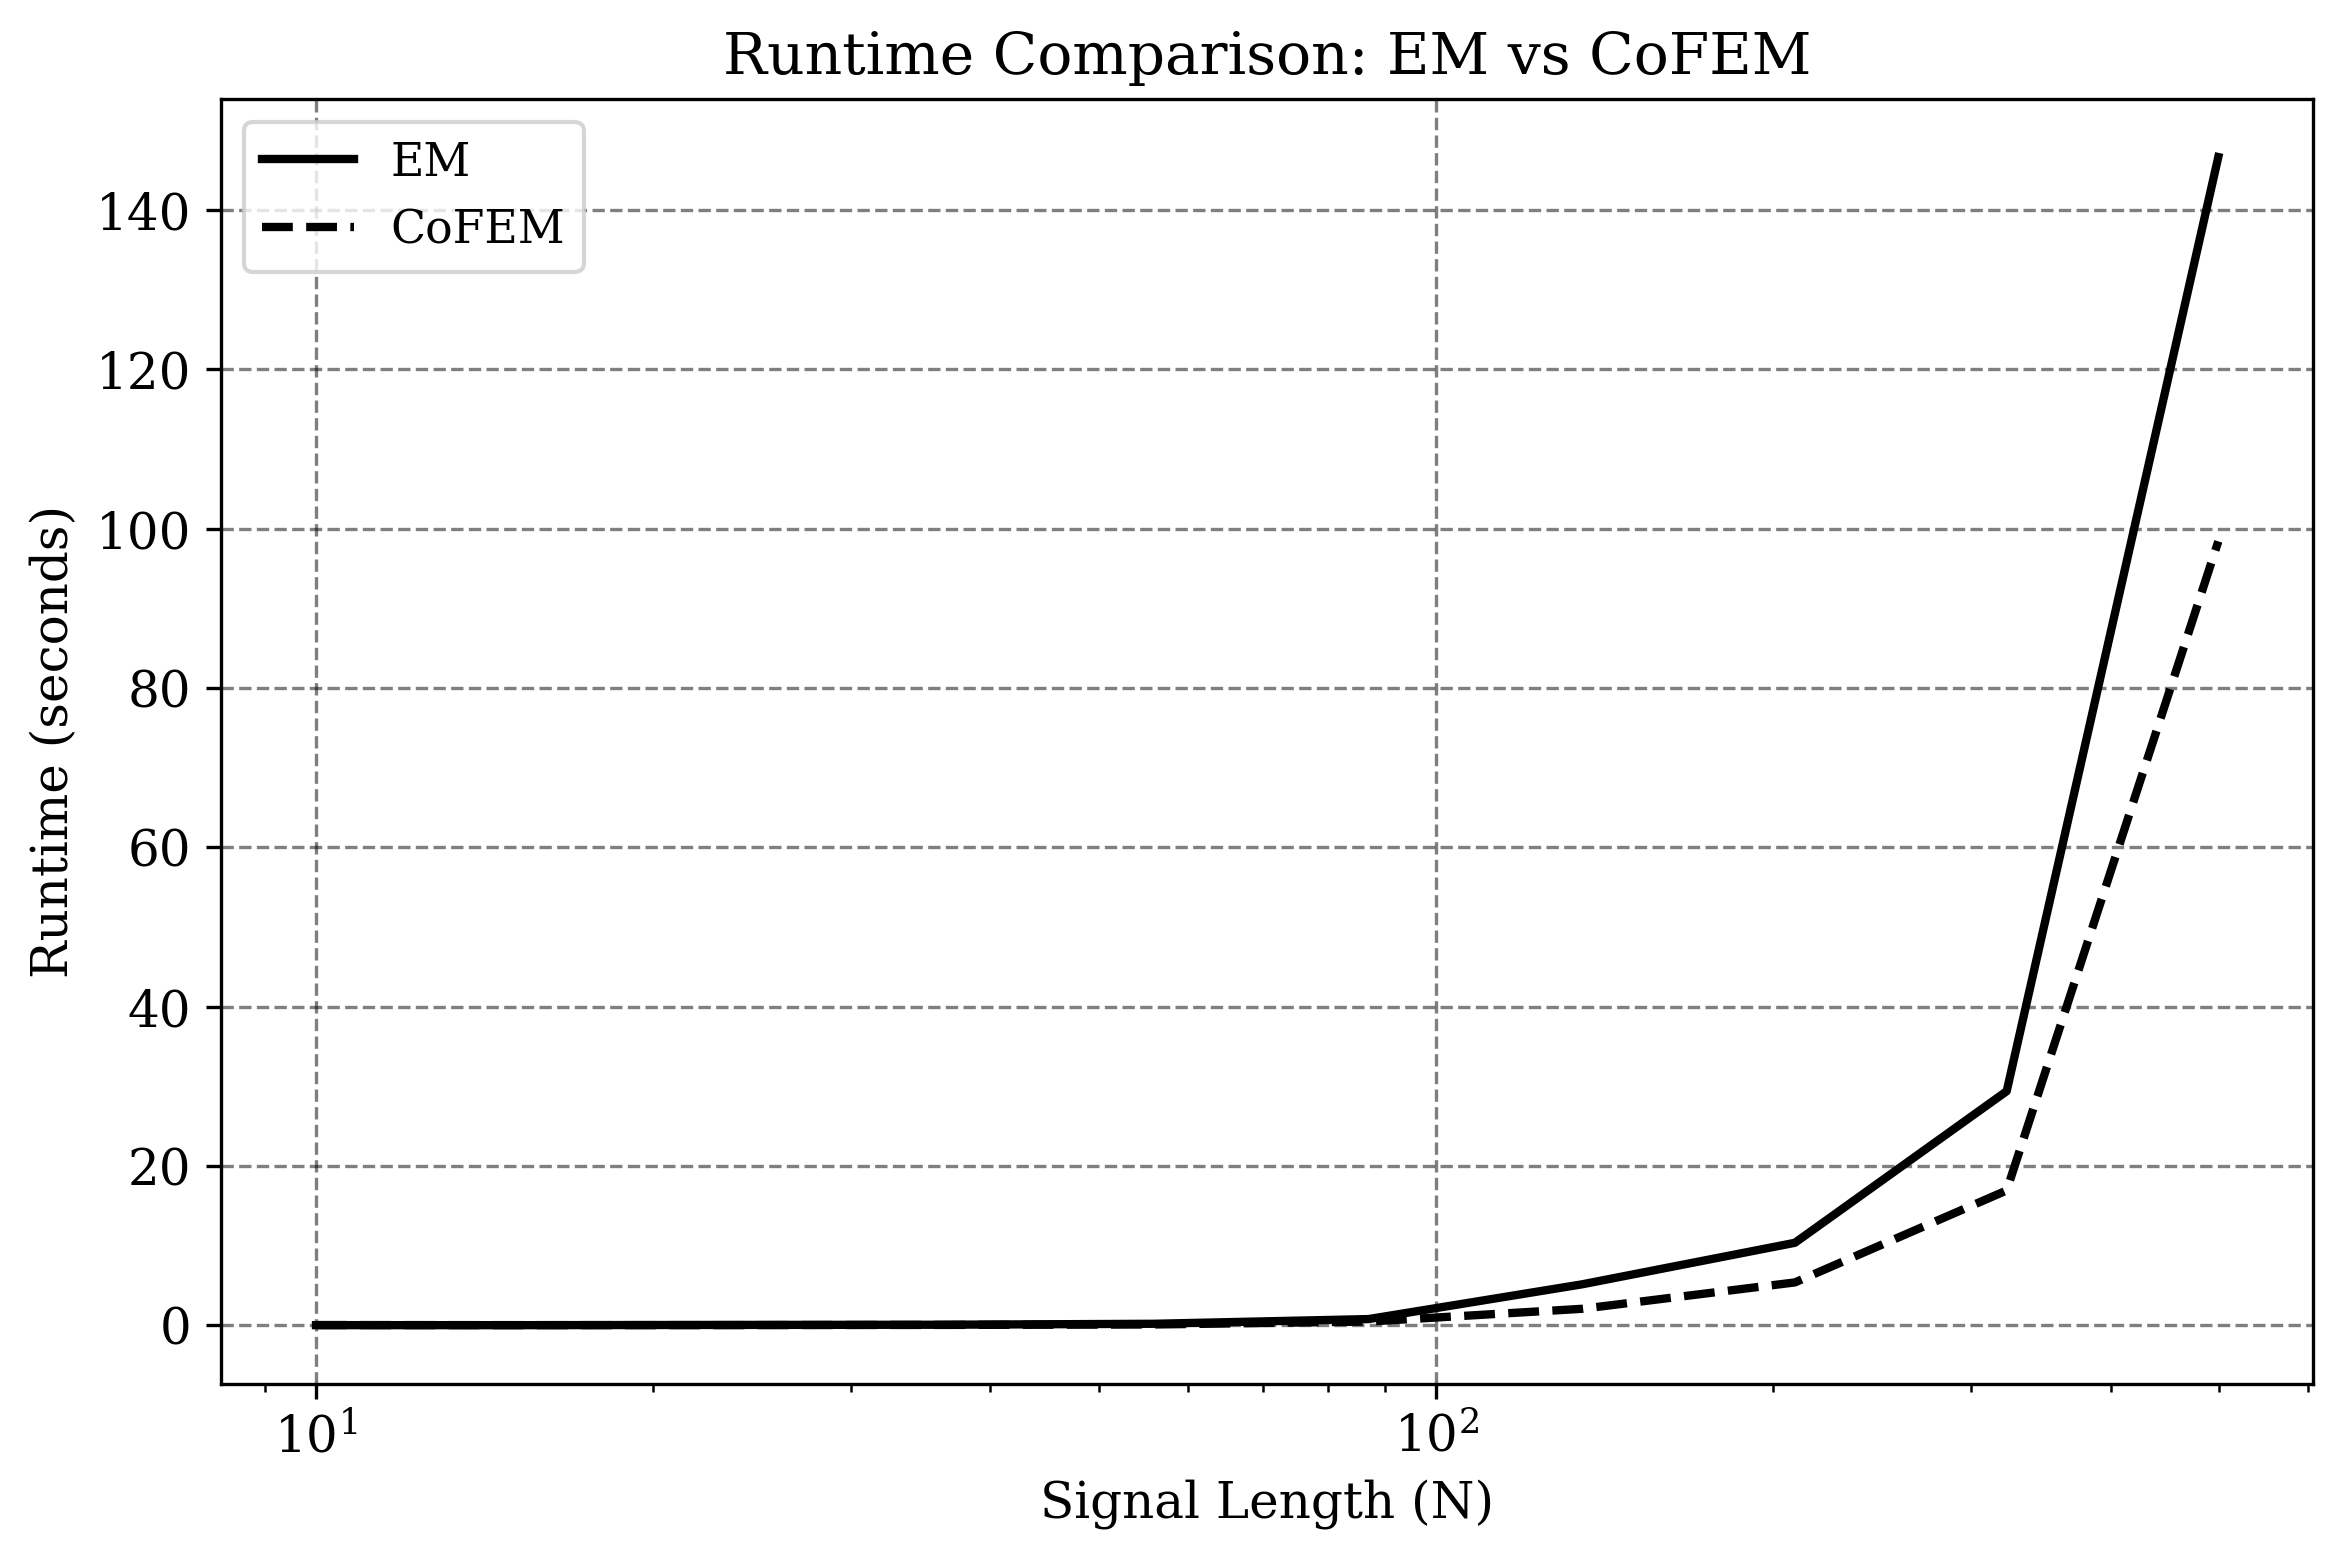
\includegraphics[width=0.75\textwidth]{Figures/runtime_comp.png}
    \caption{Runtime of the EM and CoFEM algorithms for increasing number of measurements $ N $. The dictionary size is set to $ D = 3N $.}
    \label{fig:runtime_comparison}
\end{figure}

While the CoFEM algorithm achieves a noticeable speedup over the standard EM algorithm—98.4 seconds compared to 146.6 seconds for N=500—the improvement falls short of the expected at least twofold acceleration.

\subsection{Performance Comparison of EM Algorithms}

To compare the performance of different EM-based Sparse Bayesian Learning algorithms, experiments were conducted using synthetic data generated from Gaussian dictionaries, varying both the sparsity level $ \rho $ and the undersampling factor $ \delta = N/D $. Four variants were considered: standard EM and CoFEM, each with known and unknown noise variance. The normalized root mean squared error (NRMSE) was used to evaluate reconstruction quality. Results are averaged over multiple random trials to ensure statistical robustness.

The signal dimension was fixed to $ D = 1024 $. For the sparsity analysis the undersampling factor was fixed at $ \delta = 0.25 $, corresponding to $ N = \lfloor \delta D \rfloor $ measurements. For the undersampling analysis, the sparsity level was fixed at $ \rho = 0.06 $. The measurement matrix was drawn from a standard Gaussian distribution. Additive Gaussian noise with standard deviation $ \sigma = 0.01 $ was added to the measurements. For each setting, the reported results represent the average over five random trials to account for variability due to random initialization and noise.

As shown in Figure \ref{fig:accuracy_vs_sparsity} and Figure \ref{fig:accuracy_vs_undersampling}, all four algorithms exhibit remarkably similar performance across the full range of tested sparsity and undersampling settings. In particular, the CoFEM algorithm with unknown noise variance performs on par with the variants that assume knowledge of the noise level. This observation is consistent with the findings reported in \cite{lin2022covariance}, where CoFEM and EM methods were shown to yield nearly identical reconstruction accuracy under equivalent settings.

\begin{figure}[h]
    \centering
    \includegraphics[width=0.75\linewidth]{figures/accuracy_vs_sparsity.png}
    \caption{Reconstruction accuracy (NRMSE) versus sparsity level $ \rho $. All four EM variants show near-identical behavior.}
    \label{fig:accuracy_vs_sparsity}
\end{figure}

\begin{figure}[h]
    \centering
    \includegraphics[width=0.75\linewidth]{figures/accuracy_vs_undersampling.png}
    \caption{Reconstruction accuracy (NRMSE) versus undersampling factor $ \delta $. Similar performance is observed across all algorithms.}
    \label{fig:accuracy_vs_undersampling}
\end{figure}


Given these results, and in order to simplify subsequent analysis, I choose to focus on the CoFEM algorithm with unknown noise variance in the remainder of this report. This choice is motivated by its computational scalability, the practical advantage of not requiring prior knowledge of the noise level, and the observation that its reconstruction performance closely matches that of other EM-based approaches in the tested settings. While this similarity may not generalize to all scenarios, it provides a reasonable basis for concentrating on a single representative method in this context.

Future parts of this subsection will further evaluate CoFEM performance under different dictionary types (e.g., Gaussian vs. subsampled Fourier) and analyze the impact of hyperparameters and probe strategies.

\bibliographystyle{ieeetr}   % Or another style: plain, abbrv, unsrt, etc.
\bibliography{Compressive_Sensing_Report}    

\end{document}
